\documentclass[a4paper, 10pt, oneside]{report}
\usepackage{graphicx}
\graphicspath{ {images/} }


\usepackage[textwidth = 200mm,margin = 15mm]{geometry}
\usepackage{hyperref}
\usepackage{tabularx}
\usepackage{booktabs}
\usepackage{longtable}
\setcounter{secnumdepth}{3}


\title{COS301: Application and Functional Requirements}
\date{2015-02-27}
\author{Group 3B}


\begin{document}

\maketitle
\pagenumbering{gobble}

\newpage
\pagenumbering{roman}

\tableofcontents 

\newpage
\pagenumbering{arabic}


\chapter{Introduction}

Github URL: \url{https://github.com/u12026442/group3b_men_at_work.git}
\\
\\
This document contains the architecture and functional requirements for the Buzz Discussion Board system. It will start with a brief  vision and background to explain the need for such a system from where the architecture and functional requirements will follow.


\chapter{Vision}

The user interface.
\\
\\
For the user interface we plan to make use of web application as well as a mobile application that will access that buzz system. The user will be presented with a login screen on start-up of the application. After successfully logging in the user will enter their profile. They will then receive all the groups that they are a part of and all the posts that they have not looked at will be marked. They will then be able to access the spaces, threads and replies for the groups that they are a part of as well as contribute to the groups according to their permission level.

\chapter{Background}

\textit "A general discussion of what lead to the project including potentially:"

\begin{itemize}
\item \textit business/research opportunities,
\item \textit opportunities to simplify/improve some aspect of life/work or community,
\item \textit problems your client is currently facing,
\item \textit ...
\end{itemize}

\chapter{ Functional requirements and application design}
	\section{Use case prioritization}
		\subsection{Critical}
		\subsection{Important}
		\subsection{Nice to have}
	\section{Use case/Services contracts}

\newpage
\documentclass[10pt]{article}
\usepackage{graphicx}
\graphicspath{ {images/} }


\usepackage[textwidth = 200mm,margin = 15mm]{geometry}

\usepackage{tabularx}

\begin{document}

\section{Use case: Groups}
	\subsection{Use case diagram}
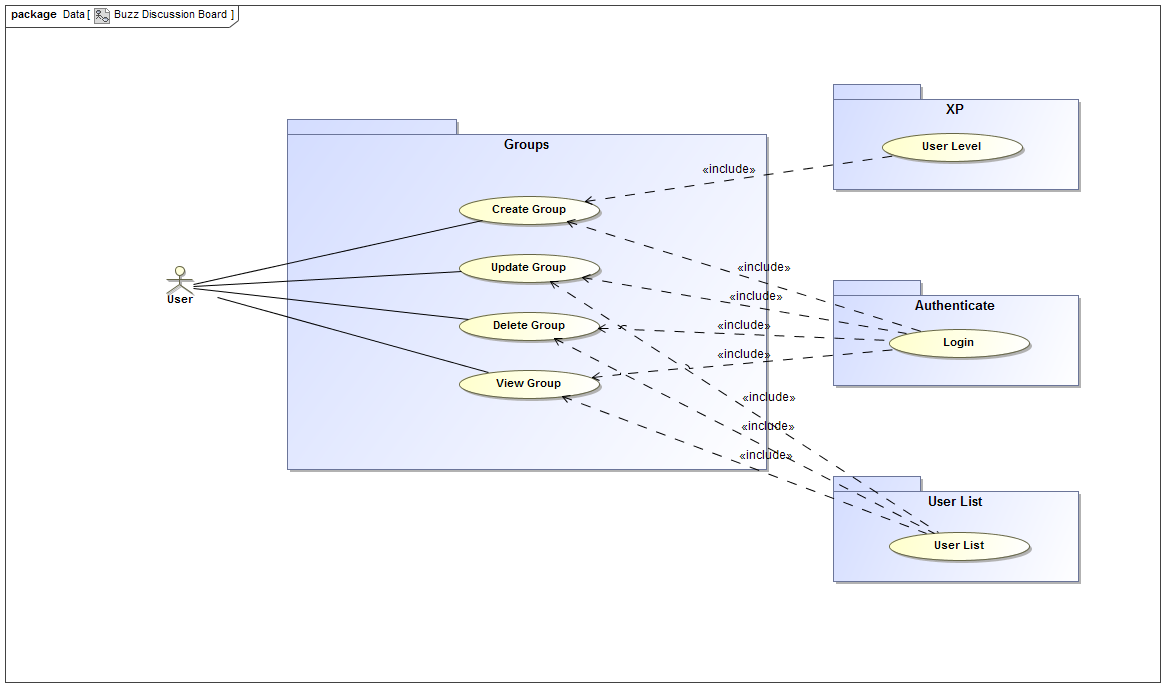
\includegraphics[width=\textwidth]{groups}
	\subsection{Short description}
	\begin{description}
		\item When a user want to create/enter a Buzz Space, first he creates a group or are part of the user-list for the group that owns the buzz space he tries to access. 
	\end{description}
	\subsection{Use cases}

\newpage
\begin{table}
\begin{tabularx}{\textwidth}{|>{\setlength\hsize{0.7\hsize}\setlength\linewidth{\hsize}}X|>{\setlength\hsize{.8\hsize}\setlength\linewidth{\hsize}}X|>{\setlength\hsize{.8\hsize}\setlength\linewidth{\hsize}}X|>{\setlength\hsize{0.7\hsize}\setlength\linewidth{\hsize}}X|}
\hline
	\multicolumn{4}{|c|}{\textbf{Use cases for Groups}}\\
\hline
	\paragraph{Use Case} & \paragraph{Preconditions} & \paragraph{Post-conditions} & \paragraph{Description} \\
\hline
	\paragraph{Create Group - User (Standard)}
&
\begin{itemize}
	\item User is logged in
	\item The group should not exist
	\item Is on XP where group creation is allowed 
\end{itemize} &
\begin{itemize}
	\item Group is created
	\item Group is saved in database
\end{itemize} &
	\paragraph{A logged in user try to create a group. Permission to create a group is dependent on the user's XP} 
	
\\
\hline
	\paragraph{Update Group}
&
\begin{itemize}
	\item User is logged in
	\item The group should exist
	\item Is part of the user-list for that group
	\item Is set to admin for the group in the user-list
\end{itemize} &
\begin{itemize}
	\item Group details is changed
	\item Changes are saved in database
	\item All members of group is notified
\end{itemize} &
	\paragraph{Changes to the group's details can only be made by the admins of the group as set out in the user-list}
\\

\hline

	\paragraph{Delete Group}
&
\begin{itemize}
	\item User is logged in
	\item The group should exist
	\item Is part of the user-list for that group
	\item Is set to admin for the group in the user-list
\end{itemize} &
\begin{itemize}
	\item Group is deleted
	\item Group is marked as deleted in database
	\item All members of group is notified
\end{itemize} &
	\paragraph{Deleting a group can only be done by the admins of the group as set out in the user-list}
\\
\hline

	\paragraph{View Group}
&
\begin{itemize}
	\item The group should exist
	\item The group should be publicly visible	
\end{itemize} &
\begin{itemize}
	\item Group details are accessed
\end{itemize} &
	\paragraph{Anyone can view the group's info if the group is a public group}
\\
\hline
	\paragraph{View Group - Hidden}
&
\begin{itemize}
	\item User is logged in
	\item The group should exist
	\item Is part of the user-list for that group
\end{itemize} &
\begin{itemize}
	\item Group details are accessed
\end{itemize} &
	\paragraph{Anyone in the group's user-list can view the group's info when the group is a hidden group}
\\
\hline


\end{tabularx}
\end{table}

\newpage
\begin{table}
\begin{tabularx}{\textwidth}{|>{\setlength\hsize{0.7\hsize}\setlength\linewidth{\hsize}}X|>{\setlength\hsize{.8\hsize}\setlength\linewidth{\hsize}}X|>{\setlength\hsize{.8\hsize}\setlength\linewidth{\hsize}}X|>{\setlength\hsize{0.7\hsize}\setlength\linewidth{\hsize}}X|}
\hline
	\multicolumn{4}{|c|}{\textbf{Use cases for Groups}}\\
\hline
	\paragraph{Use Case} & \paragraph{Preconditions} & \paragraph{Post-conditions} & \paragraph{Description} \\
	\paragraph{Create Group - User (Admin)}
&
\begin{itemize}
	\item User is logged in as Admin
	\item The group should not exist
\end{itemize} &
\begin{itemize}
	\item Group is created
	\item Group is saved in database
\end{itemize} &
	\paragraph{A logged in Admin can add a group. } 
	
\\
\hline
	\paragraph{Update Group - Admin}
&
\begin{itemize}
	\item User is logged in as Admin
	\item The group should exist
\end{itemize} &
\begin{itemize}
	\item Group details is changed
	\item Changes are saved in database
	\item All members of group is notified
\end{itemize} &
	\paragraph{Changes to the group's details can only be made by the admins of the buzz system}
\\

\hline

	\paragraph{Delete Group - Admin}
&
\begin{itemize}
	\item User is logged in as Admin
	\item The group should exist
\end{itemize} &
\begin{itemize}
	\item Group is deleted
	\item Group is marked as deleted in database
	\item All members of group is notified
\end{itemize} &
	\paragraph{Deleting a group can be done by the admins of the buzz system}
\\
\hline





\end{tabularx}
\end{table}


\end{document}
\newpage
	\section{Use case: Spaces}
	\subsection{Use case diagram}
	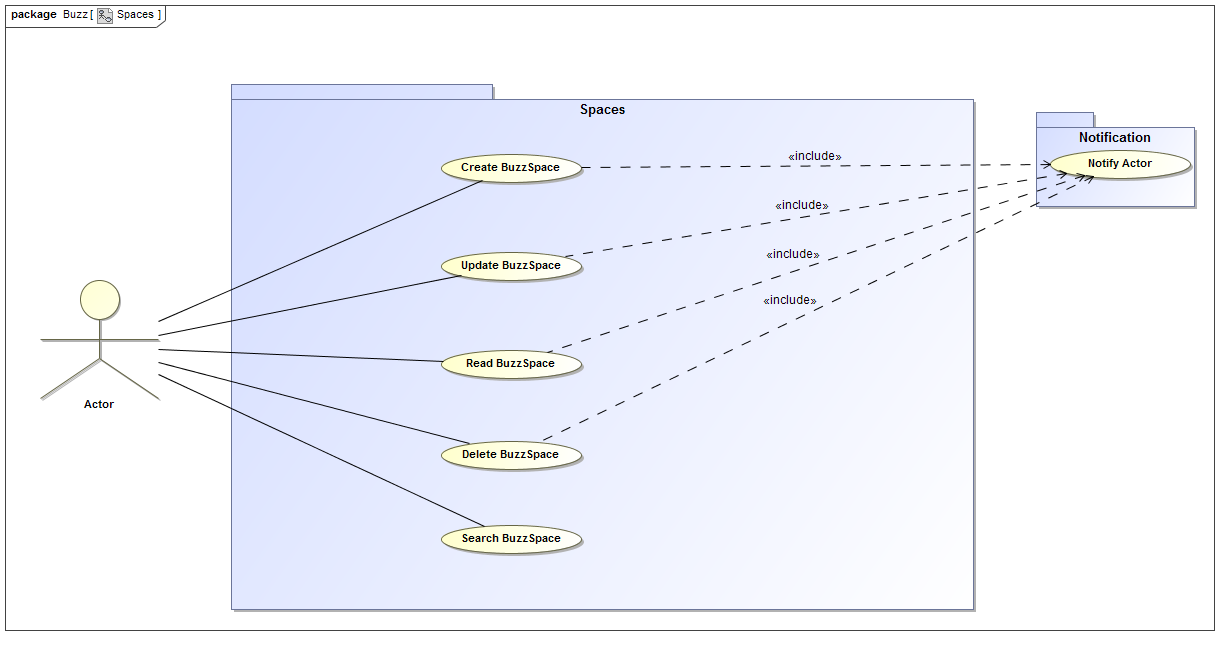
\includegraphics[width=\textwidth]{spacesUseCase}
	\subsection{Short description}
	\begin{description}
		
		\item[] 
			The following section will discuss the functional requirements of the Spaces section of the BuzzSpace program.
		
		\item[] Different actors:
		\begin{itemize}
			\item Administrator: Has system wide permission.
			\item Lecturer: Has full permission for the current BuzzSpace
			\item User: Has permission for the current BuzzSpace according to the users XP. Lecturer will included in users as they will be assigned the required XP.   
		\end{itemize}
		
	\end{description}
	
	\subsection{Use case prioritization}
	\begin{description}
		\item[] Critical
		\begin{itemize}
			\item Create BuzzSpace
			\item Delete BuzzSpace
			\item Update BuzzSpace
			\item Read BuzzSpace
			\item Authentication
		\end{itemize}
		
		\item[] Important
		\begin{itemize}
			\item Search BuzzSpaces
			\item Check XP
		\end{itemize}
	\end{description}
	
	\subsection{Use cases}
	\newpage
	\begin{longtable}{@{}|p{1.5cm}|p{2.2cm}|p{3cm}|p{3.5cm}|p{3.5cm}|@{}}
		\toprule
		\multicolumn{5}{|c|}{\textbf{Use cases for Space}}\\
		\hline
		\textbf{Actor} & \textbf{Use Case} & \textbf{Pre-condition} & \textbf{Post-Conditions} & \textbf{Description} \\ \midrule
		
		User Or Admin& 
		Create BuzzSpace& 
		\begin{itemize}
			\item A group must exist
			\item The actor has permission
			\item The actor has the required amount of XP
		\end{itemize}& 
		\begin{itemize}
			\item Space created
		\end{itemize} & 
		Create a new BuzzSpace (discussion space within group) \\ \midrule
		
		User Or Admin& 
		Delete BuzzSpace& 
		\begin{itemize}
			\item The BuzzSpace exists that wants to be removed
			\item The actor has permission
			\item The actor has the required amount of XP
		\end{itemize}& 
		\begin{itemize}
			\item BuzzSpace removed from groups
		\end{itemize} & 
		Remove a BuzzSpace from groups and notify the users belonging to that group \\ \midrule
		
		User Or Admin& 
		Update BuzzSpace& 
		\begin{itemize}
			\item The Space exists that needs to be updated
			\item The actor has permission
			\item The actor has the required amount of XP
		\end{itemize}& 
		\begin{itemize}
			\item State of space changed
		\end{itemize} & 
		Allow users with permission to update the BuzzSpace \\ \midrule
		
		User Or Admin& 
		Read BuzzSpace& 
		\begin{itemize}
			\item The Space exists
			\item The actor has permission
		\end{itemize}& 
		\begin{itemize}
			\item BuzzSpace marked read
		\end{itemize} & 
		Allow users with permission to read the BuzzSpaces \\ \midrule
		
		User Or Admin& 
		Search BuzzSpaces& 
		\begin{itemize}
			\item Must be a registered user
		\end{itemize}& 
		\begin{itemize}
			\item Search list created
		\end{itemize} & 
		Search the BuzzSpaces in groups \\ \midrule
		
		User Or Admin& 
		Authentication& 
		\begin{itemize}
			\item Actor must be registered
			\item Actor must be logged into the Buzz System 
		\end{itemize}& 
		\begin{itemize}
			\item Actor grated access
		\end{itemize} & 
		See if the Actor is authenticated to the system \\ \midrule
		
		User Or Admin& 
		Check XP& 
		\begin{itemize}
			\item Actor must be registered
			\item Actor must be logged into the Buzz System 
			\item Actor has the required amount of XP
		\end{itemize}& 
		\begin{itemize}
			\item Actor allowed to make changes
		\end{itemize} & 
		See if the Actor has the required amount of XP to be allowed to make changes to the BuzzSpace \\ \bottomrule
		
	\end{longtable}
\newpage


\section{Use case: Threads and replies}
	\subsection{Use case diagram}
	\begin{description}
		\item[Use case diagram for threads.] 
	\end{description}
	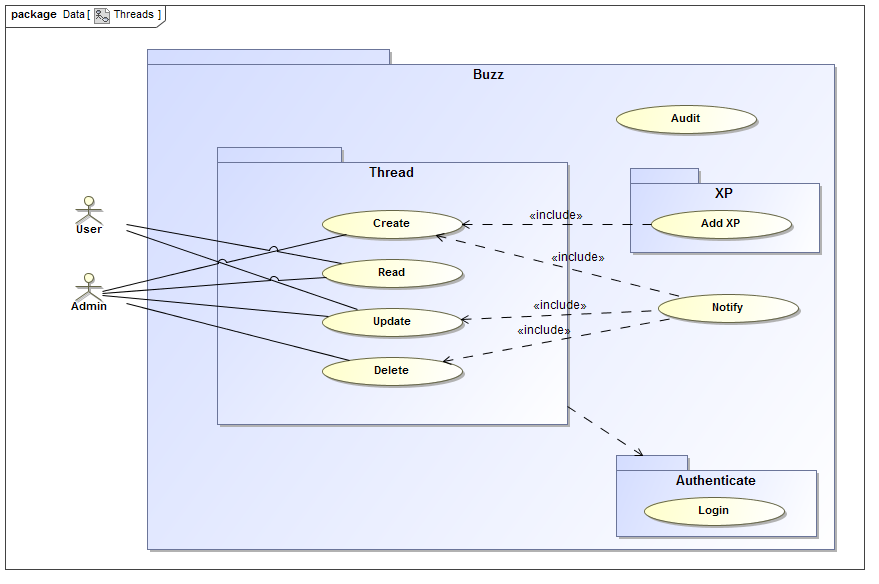
\includegraphics[width=\textwidth]{Threads}
\newpage
		\begin{description}
			\item[Use case diagram for replies.] 
		\end{description}
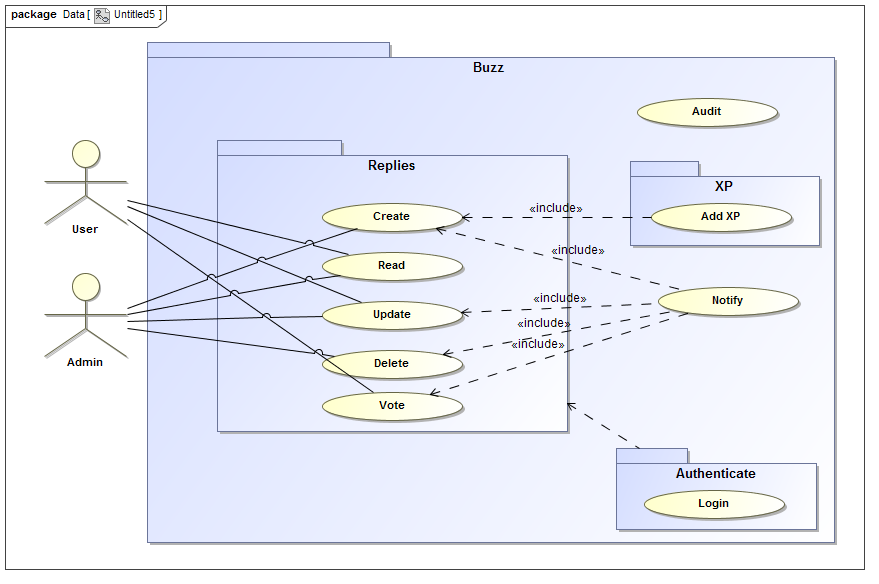
\includegraphics[width=\textwidth]{Replies}
	
	\subsection{Short description}
	\begin{description}
		\item[Above diagrams depicts the relationships between different components for ]
		 \item[the thread and reply systems within Buzz.] 
	\end{description}
	\subsection{Use cases}


\begin{table}
\begin{tabularx}{\textwidth}{|>{\setlength\hsize{0.5\hsize}\setlength\linewidth{\hsize}}X|>{\setlength\hsize{.8\hsize}\setlength\linewidth{\hsize}}X|>{\setlength\hsize{.9\hsize}\setlength\linewidth{\hsize}}X|>{\setlength\hsize{0.8\hsize}\setlength\linewidth{\hsize}}X|}
\hline
	\multicolumn{4}{|c|}{\textbf{Use cases for: Threads and Replies}}\\
\hline
	\paragraph{Use Case} & \paragraph{Precondition} & \paragraph{Post-condition} & \paragraph{Description} \\
\hline
	\paragraph{Create Thread}
&
\begin{itemize}
	\item Creator must be authenticated and  logged in
	\item Creator must have the necessary privileges to create a topic in the current space
	\item Creator must belong to a group
	
	
\end{itemize} &
\begin{itemize}
\item	Thread contains a subject or title
\item	Thread contains a clear short description 
\item	Thread shows the author
\item	Thread shows status(Published /Unpublished)
\item	Thread contains descriptive tags
\item	Thread shows total replies (if any available)
\item	Thread belongs to a category
\item	Thread has a valid date
\item	Thread allows for users to rate it
\item Thread is saved to database
\item All relevant users are notified of the existence of the thread
\item Creator of thread recieves Xp

\end{itemize} &
	\paragraph{Creates a thread within a space with the neccesary information}
\\
\hline
	\paragraph{Create Reply}
	&
	\begin{itemize}
\item	User  must be authenticated and  logged in
\item	User must belong to a group
\item	User must be able to participate in threads within current space
\item	A thread must exist
	
		
		
	\end{itemize} &
	\begin{itemize}
\item Reply post is linked to the right thread
\item Reply is in correct format
\item Reply is in correct format
\item Reply is saved to database
	\item All relevant users are notified that a reply has been posted

	\end{itemize} &
	\paragraph{Creates a reply thats part of a thread}
	\\
	\hline
		\paragraph{Delete Thread}
		&
		\begin{itemize}
			\item	User  must be authenticated and  logged in
			\item	User must belong to a group
			\item	A thread must exist
			\item  user must have the necessary privileges(or Xp) to delete a thread in the current space
			
			
			
		\end{itemize} &
		\begin{itemize}
			\item Thread is deleted
			\item All relevant users are notified that the thread is deleted
		
			
		\end{itemize} &
		\paragraph{A thread is deleted}
		\\
	\hline
\end{tabularx}
\end{table}
\newpage
\begin{table}
	\begin{tabularx}{\textwidth}{|>{\setlength\hsize{0.5\hsize}\setlength\linewidth{\hsize}}X|>{\setlength\hsize{.8\hsize}\setlength\linewidth{\hsize}}X|>{\setlength\hsize{.9\hsize}\setlength\linewidth{\hsize}}X|>{\setlength\hsize{0.8\hsize}\setlength\linewidth{\hsize}}X|}
		\hline
		\multicolumn{4}{|c|}{\textbf{Use cases for: Threads and Replies}}\\
		\hline
		\paragraph{Use Case} & \paragraph{Precondition} & \paragraph{Post-condition} & \paragraph{Description} \\
		\hline
		\paragraph{Delete Reply}
		&
		\begin{itemize}
				\item	User  must be authenticated and  logged in
				\item	User must belong to a group
				\item	A thread must exist
				\item  user must have the necessary privileges(or Xp) to delete a thread in the current space
				
			
			
		\end{itemize} &
		\begin{itemize}
			\item Reply is deleted
				\item All relevant users are notified that a reply has been deleted
				
			
			
			
		\end{itemize} &
		\paragraph{Delete a reply}
		\\
			\hline
			\paragraph{Update Thread}
			&
			\begin{itemize}
				\item	User  must be authenticated and  logged in
				\item	User must belong to a group
				\item	A thread must exist
				\item  user must have the necessary privileges(or Xp) to update a thread in the current space
				
				
				
			\end{itemize} &
			\begin{itemize}
				\item Thread is updated
				\item Thread is saved to the database
						\item All relevant users are notified that an update to a thread has been made
						
				
				
				
			\end{itemize} &
			\paragraph{User updates a thread}
			\\
			\hline
			
				\paragraph{Update Reply}
				&
				\begin{itemize}
					\item	User  must be authenticated and  logged in
					\item	User must belong to a group
					\item	A thread must exist
					\item  user must have the necessary privileges(or Xp) to update a reply in the current space
					
					
					
				\end{itemize} &
				\begin{itemize}
					\item Thread is updated
					\item Thread is saved to the database
						\item All relevant users are notified that an update to a reply has been made
					
					
					
				\end{itemize} &
				\paragraph{User updates a reply}
				\\
				\hline
	

	\end{tabularx}
\end{table}
\newpage
\begin{table}
	\begin{tabularx}{\textwidth}{|>{\setlength\hsize{0.5\hsize}\setlength\linewidth{\hsize}}X|>{\setlength\hsize{.8\hsize}\setlength\linewidth{\hsize}}X|>{\setlength\hsize{.9\hsize}\setlength\linewidth{\hsize}}X|>{\setlength\hsize{0.8\hsize}\setlength\linewidth{\hsize}}X|}
		\hline
		\multicolumn{4}{|c|}{\textbf{Use cases for: Threads and Replies}}\\
		\hline
		\paragraph{Use Case} & \paragraph{Precondition} & \paragraph{Post-condition} & \paragraph{Description} \\
		\hline
	
		\paragraph{Read a Thread}
		&
		\begin{itemize}
			\item	User  must be authenticated and  logged in
			\item	User must belong to a group
			\item	User must be able to participate in threads within current space
			\item	A thread must exist
			
			
			
		\end{itemize} &
		\begin{itemize}
		\item Thread status is updated to read for the current user
			
		\end{itemize} &
		\paragraph{User reads a thread}
		\\
		\hline
		\paragraph{Read a reply}
		&
		\begin{itemize}
			\item	User  must be authenticated and  logged in
			\item	User must be able to participate in threads within current space
			\item	A thread must exist
		
			
			
		\end{itemize} &
		\begin{itemize}
	\item Reply status is updated to read for the current user
			
			
		\end{itemize} &
		\paragraph{User reads a reply}
		\\
			\hline
			\paragraph{Vote}
			&
			\begin{itemize}
				\item	User  must be authenticated and  logged in
				\item	User must be able to participate in threads and replies within current space
		
				
				
			\end{itemize} &
			\begin{itemize}
				\item A vote has been made to a thread or reply.
				
				
			\end{itemize} &
			\paragraph{Users vote for threads and replies based on the relevance of the content}
			\\
			\hline
	\end{tabularx}
\end{table}

\newpage
\include{replies}
\newpage
\include{user}
\newpage
\documentclass{article}
\usepackage{graphicx}
\graphicspath{ {images/} }

\usepackage[textwidth = 195mm]{geometry}
\usepackage{tabularx}

\begin{document}

\section{Use case: Threads and replies}
	\subsection{Use case diagram}
	\subsection{Short description}
	\begin{description}
		\item[Depicts the functionality for buzz system through use cases.] 
	\end{description}
	\subsection{Use cases}

\newpage
\begin{table}
\begin{tabularx}{\textwidth}{|>{\setlength\hsize{0.5\hsize}\setlength\linewidth{\hsize}}X|>{\setlength\hsize{.8\hsize}\setlength\linewidth{\hsize}}X|>{\setlength\hsize{.9\hsize}\setlength\linewidth{\hsize}}X|>{\setlength\hsize{0.8\hsize}\setlength\linewidth{\hsize}}X|}
\hline
	\multicolumn{4}{|c|}{\textbf{Use cases for: Threads and Replies}}\\
\hline
	\paragraph{Use Case} & \paragraph{Precondition} & \paragraph{Post-condition} & \paragraph{Description} \\
\hline
	\paragraph{Create User List}
&
\begin{itemize}
	\item User creating the list is logged in and has permission to create a user list.
	\item A group exists to accept the user list.
	
\end{itemize} &
\begin{itemize}
\item	New user list is created.
\item The user list is assigned to the group.

\end{itemize} &
	\paragraph{Creates a new user list and assigns it to a group}
\\
\hline
	\paragraph{Update the user list}
	&
	\begin{itemize}
\item	User updateing the list is logged in and has permission to update the user list.
\item	The user list being updated exists.
	
		
		
	\end{itemize} &
	\begin{itemize}
\item User is added to the user list.
\item	The user is notified that they have been added.

	\end{itemize} &
	\paragraph{Adding users to the user list}
	\\
	\hline
	\paragraph{Set user permission}
	&
	\begin{itemize}
		\item User setting the permission is logged in and has permission to set permissions for that user list.
		\item User having their permissions changed is a member of that user list.
		
	\end{itemize} &
	\begin{itemize}
		\item	The user whos permissions have been changed is notified of the change.
		\item The new permission level is saved to the database.
		\item User has access to the functionallity assigned to that permission level.
		
	\end{itemize} &
	\paragraph{Sets the permission for a user in the user list.}
	\\
	\hline
\end{tabularx}
\end{table}

\newpage
\begin{table}
	\begin{tabularx}{\textwidth}{|>{\setlength\hsize{0.5\hsize}\setlength\linewidth{\hsize}}X|>{\setlength\hsize{.8\hsize}\setlength\linewidth{\hsize}}X|>{\setlength\hsize{.9\hsize}\setlength\linewidth{\hsize}}X|>{\setlength\hsize{0.8\hsize}\setlength\linewidth{\hsize}}X|}
		\hline
		\multicolumn{4}{|c|}{\textbf{Use cases for: Threads and Replies}}\\
		\hline
		\paragraph{Use Case} & \paragraph{Precondition} & \paragraph{Post-condition} & \paragraph{Description} \\
		\hline
		\paragraph{Get user list}
		&
		\begin{itemize}
			\item The user making the request is logged in and has permission to access the user list.
			\item User User list exists.
			\item The user is trying to access the user list assigned to the group he is in.
			
		\end{itemize} &
		\begin{itemize}
			\item	User making the request gets the list of users in the user list.
			
		\end{itemize} &
		\paragraph{Retrieving the list of users in the user list.}
		\\
		\hline
		\paragraph{Add user.}
		&
		\begin{itemize}
			\item	User performing the add is logged in and has permission to update the user list.
			\item	The user list being updated exists.
			\item The user being added is a registered user.
			
			
			
		\end{itemize} &
		\begin{itemize}
			\item User being added is included into the user list.
			\item The user that is added is notified of the addition.
			\item User now has access to the information with in that group.
			
		\end{itemize} &
		\paragraph{Adding users to the user list}
		\\
		\hline
		\paragraph{Remove user}
		&
		\begin{itemize}
			\item User performing the update is logged in and has permission to update that user list.
			\item User being removed is a member of that user list.
			
		\end{itemize} &
		\begin{itemize}
			\item	The user being removed from the list is no longer a member of the user list.
			\item The user being removed is notified of the change.
			
		\end{itemize} &
		\paragraph{Removing a user from the user list.}
		\\
		\hline
		\paragraph{Remove user list}
		&
		\begin{itemize}
			\item User performing the update is logged in and has permission to update that user list.
			\item User list being removed exists.
			
		\end{itemize} &
		\begin{itemize}
			\item	The users being removed from the list is no longer a member of the user list.
			\item The user being removed is notified of the change.
			\item the user list is deleted
			
		\end{itemize} &
		\paragraph{Removing the entire user list.}
		\\
		\hline
	\end{tabularx}
\end{table}

\end{document}
\newpage
\include{userinterface}
\newpage
%\documentclass[a4paper, 10pt, oneside]{report}
\usepackage{graphicx}
\graphicspath{ {images/} }


\usepackage[textwidth = 200mm,margin = 15mm]{geometry}
\usepackage{hyperref}
\usepackage{tabularx}
\usepackage{booktabs}
\usepackage{longtable}
\setcounter{secnumdepth}{3}


\title{COS301: Application and Functional Requirements}
\date{2015-02-27}
\author{Group 3B}


\begin{document}

	\section{Use case: Spaces}
	\subsection{Use case diagram}
	%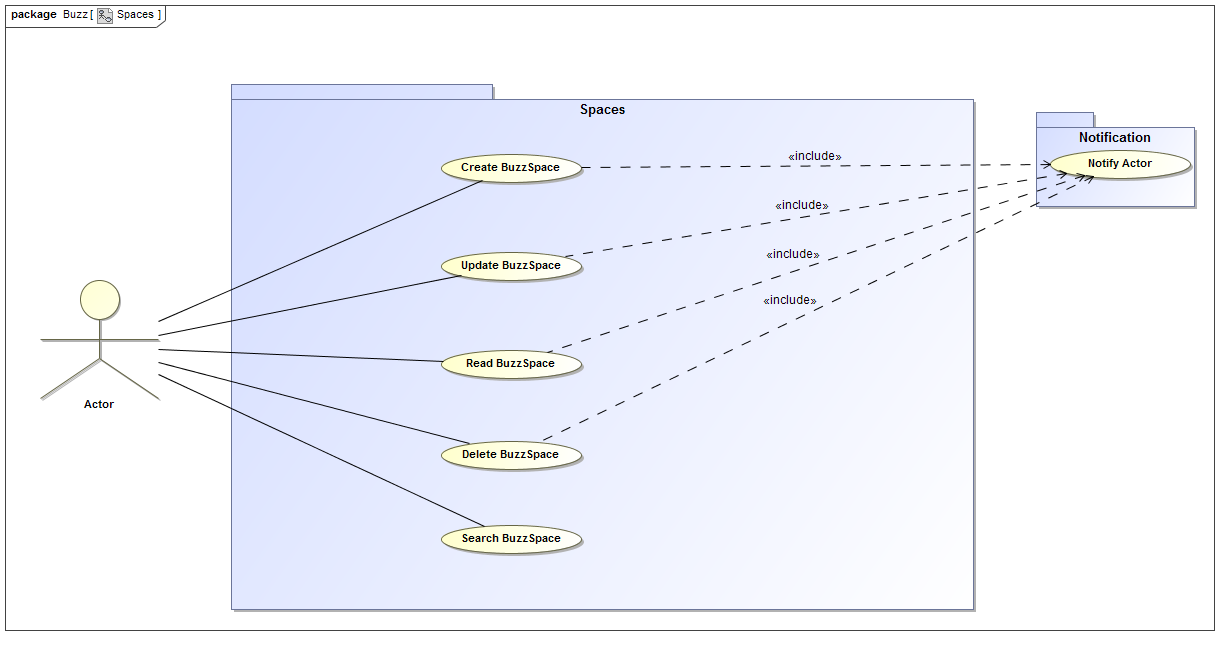
\includegraphics[width=\textwidth]{spacesUseCase}
	\subsection{Short description}
	\begin{description}
		
		\item[] 
			This section is for authentication relating to logging into the Buzz system and logging out of the system.
		
		\item[] Different actors:
		\begin{itemize}
			\item Administrator.
			\item User.   
		\end{itemize}
		
	\end{description}
	
	\subsection{Use case prioritization}
	\begin{description}
		\item[] Critical
		\begin{itemize}
			\item Login
			\item Logout
		\end{itemize}
	\end{description}
	
	\subsection{Use cases}
	\newpage
	\begin{longtable}{@{}|p{1.5cm}|p{2.2cm}|p{3cm}|p{3.5cm}|p{3.5cm}|@{}}
		\toprule
		\multicolumn{5}{|c|}{\textbf{Use cases for Space}}\\
		\hline
		\textbf{Actor} & \textbf{Use Case} & \textbf{Pre-condition} & \textbf{Post-Conditions} & \textbf{Description} \\ \midrule
		
		User Or Admin& 
		Login& 
		\begin{itemize}
			\item Buzz system must exist.
			\item User and administrator must be registered to use Buzz system.
		\end{itemize}& 
		\begin{itemize}
			\item User or admin will be logged into Buzz system.
		\end{itemize} & 
		User or admin logs into Buzz system. \\ \midrule
		
		User Or Admin& 
		Logout& 
		\begin{itemize}
			\item User and admin must be logged in.
		\end{itemize}& 
		\begin{itemize}
			\item User or admin will be logged out.
		\end{itemize} & 
		User or admin can log out of Buzz system \\ \bottomrule
		
		
		
	\end{longtable}
\end{document
%\newpage
\include{audit}
\newpage
\include{report}
\newpage
\documentclass{article}
\usepackage{graphicx}
\graphicspath{ {images/} }

\usepackage[textwidth = 155mm]{geometry}

\begin{document}

\section{Use case: XP}
	\subsection{Use case diagram}
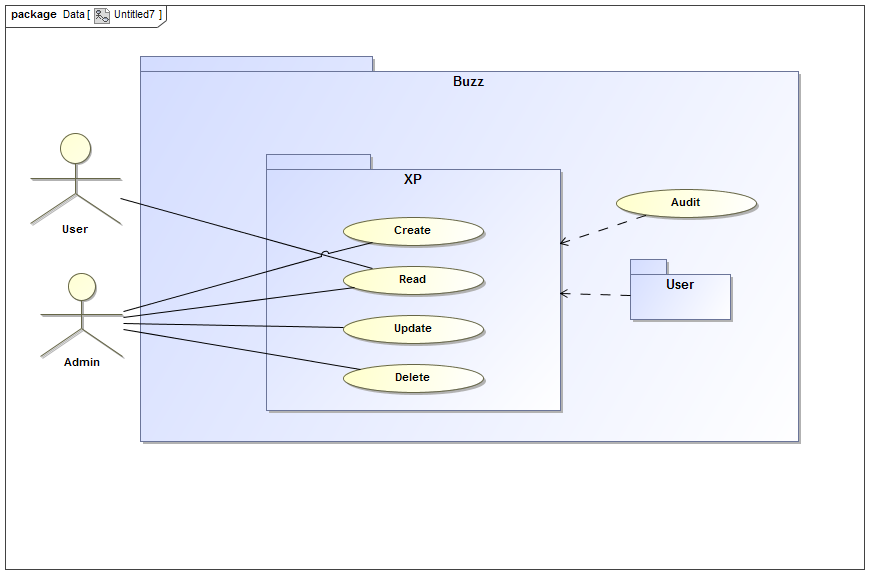
\includegraphics[width=\textwidth]{XP.png}
	\subsection{Description}
	\begin{description}
		\item[] This is the use case table for XP (User levels). The levels are set by the administrator. User's level may change when their participation meets the criteria for a particular level.  
	\end{description}
	\subsection{Use case table}

\newpage
 \begin{table}
 	\begin{tabular}{p{3cm}p{3cm}p{3cm}p{3cm}p{3cm}}
 		\hline
 		Actor & Use-Case & Description & Pre-condition & Post-condition \\ \hline
 		Administrator & Update to rock level & Assign buzz space user lowest level & User must be a registered student & User is assigned rock level and can post threads and reply to threads.\\ \hline
 		Administrator & Update to bronze level & Promote user from rock level to bronze level. & User must have posted 20 threads and replied 100 times to multiple threads.  & User moves from rock level to bronze level. User will be able to report inappropriate threads and replies.\\ \hline
 		Administrator & Update to silver level & Promote user from bronze level to silver level. & User must have posted 60 threads and replied 200 times to multiple threads. & User moves from bronze level to silver level. User will be able to delete threads or replies that have been reported as inappropriate. \\ \hline
 		Administrator & Update to gold level & Promote user from silver level to gold level. & User must have posted 100 threads and replied 350 times to multiple threads. & User moves from silver level to gold level. User will be able to delete threads and replies, whether they have been reported or not. \\ \hline
 		Administrator & Update to black diamond level & Promote user from gold level to black diamond level. & User must have posted 120 threads and replied 450 timesto multiple threads. & User moves from gold level to black diamond level. User will be able to delete/archive threads and replies  \\ \hline
 		Administrator & Update to platinum level & Promote user from black diamond level to platinum level. & User must have posted 200 threads and replied 600 times to multiple threads. & User moves from black diamond level to platinum level. User will be able to delete/archive threads and replies. User will be able to send warnings to buzz space users if there’s misconduct. \\ \hline  Administrator & Assign titanium level to user & Promote user from platinum level to titanium level. & User must have posted 400 threads and replied 800 times to multiple threads. & User moves from platinum level titanium level. User will be able to delete/archive threads and replies. User will be able to ban buzz space users if there’s misconduct. \\ \hline 
 		User &  View level status & Buzz space user will be able to view their progress and outstanding requirements to advance to the next level. & User must be assigned to a level. & User views their buzz space level in status bar form, and outstanding requirements to the next level. \\ \hline
 	\end{tabular}
 \end{table}



\end{document}

\newpage

\section{Required functionality}
\section{Process specifications}
\section{Domain Model}
\section{Open Issues}



\end{document}

